%
% main.tex
%
% Copyright (C) 2020 by SpaceLab.
%
% PC-104 Adapter Documentation
%
% This work is licensed under the Creative Commons Attribution-ShareAlike 4.0
% International License. To view a copy of this license,
% visit http://creativecommons.org/licenses/by-sa/4.0/.
%

%
% \brief Main file.
%
% \author Gabriel Mariano Marcelino <gabriel.mm8@gmail.com>
%
% \institution Universidade Federal de Santa Catarina (UFSC)
%
% \version 2.0.0
%
% \date 2020/06/21
%

\documentclass[a4paper,12pt]{book}

\usepackage{spacelab_book}

\title{PC-104 Adapter Documentation}
\author{SpaceLab}
\date{\today}

% File metadata
\hypersetup
{
    pdfauthor   = {SpaceLab},
    pdfsubject  = {\thetitle},
    pdftitle    = {\thetitle},
    pdfkeywords = {Nanosatellites, Cubesats, GOLDS-UFSC}
}

\begin{document}

    \pagenumbering{roman}
    \setcounter{page}{1}

    %
% titlepage.tex
%
% Copyright (C) 2020 by SpaceLab.
%
% PC-104 Adapter Documentation
%
% This work is licensed under the Creative Commons Attribution-ShareAlike 4.0
% International License. To view a copy of this license,
% visit http://creativecommons.org/licenses/by-sa/4.0/.
%

%
% \brief Title page.
%
% \author Gabriel Mariano Marcelino <gabriel.mm8@gmail.com>
%
% \institution Universidade Federal de Santa Catarina (UFSC)
%
% \version 0.1.0
%
% \date 2020/06/21
%

\begin{titlepage}

\thispagestyle{empty}

\begin{flushleft}
SPACELAB.PC104-ADAPTER.2020.06.001 REV A. ISSUE 0.1
\end{flushleft}

\begin{figure}[!ht]
    \begin{flushleft}
        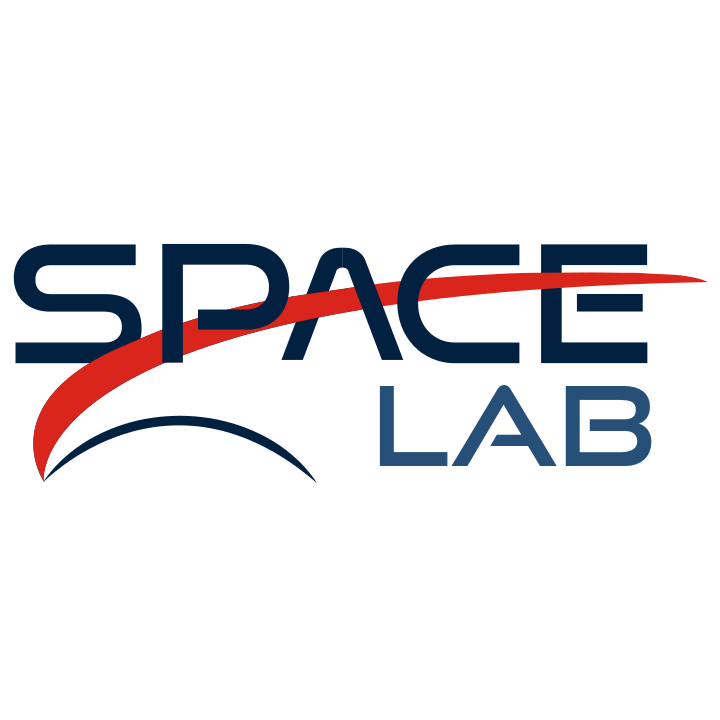
\includegraphics[width=5cm]{figures/spacelab.png}
    \end{flushleft}
\end{figure}

\begin{flushleft}
\Huge{\textbf{\thetitle}}
\rule[0pt]{\textwidth}{5pt}
\end{flushleft}

\vspace{0.2cm}

\begin{flushleft}
\textit{\thetitle} \\
\textit{SpaceLab, Universidade Federal de Santa Catarina, Florianópolis - Brazil}
\end{flushleft}

\vfill
\vfill

\begin{flushright}
June 2020
\end{flushright}

\end{titlepage}

    \cleardoublepage
    %
% authorpage.tex
%
% Copyright (C) 2023 SpaceLab.
%
% PC-104 Adapter Documentation
%
% This work is licensed under the Creative Commons Attribution-ShareAlike 4.0
% International License. To view a copy of this license,
% visit http://creativecommons.org/licenses/by-sa/4.0/.
%

%
% \brief Author page.
%
% \author Gabriel Mariano Marcelino <gabriel.mm8@gmail.com>
%
% \institution Universidade Federal de Santa Catarina (UFSC)
%
% \version 2.1.0
%
% \date 2020/06/21
%

\thispagestyle{empty}

\begin{center}

\textbf{\thetitle}

\textit{November, 2023}

\vspace{1cm}

\textbf{Project Chief:}

Eduardo Augusto Bezerra

\vspace{1cm}

\textbf{Authors:}

Gabriel Mariano Marcelino \\

\vspace{1cm}

\textbf{Contributing Authors:}

André Martins Pio de Mattos \\
Edemar Morsch Filho \\
Yan Castro Azeredo \\

\vspace{1cm}


\textbf{Revision Control:}

\end{center}

\begin{table}[!ht]
    \begin{center}
        \begin{tabular}{cL{5cm}L{5.5cm}C{2cm}}
            \toprule[1.5pt]
            \textbf{Version} & \textbf{Author}  & \textbf{Changes}    & \textbf{Date} \\
            \midrule
            0.1     & Gabriel M. Marcelino      & Document creation   & 2020/06/21 \\
            2.0     & Gabriel M. Marcelino      & First release       & 2020/12/26 \\
            2.1     & Gabriel M. Marcelino      & Minor fixes         & 2023/11/17 \\
                    &                           &                     &            \\
                    &                           &                     &            \\
            \bottomrule[1.5pt]
        \end{tabular}
    \end{center}
\end{table}

\vfill

\begin{figure}[!h]
	\begin{center}
		\includegraphics[width=0.25\textwidth]{figures/by-sa.eps}
	\end{center}
\end{figure}

\textcopyright\  2023 by SpaceLab. \thetitle. This work is licensed under the Creative Commons Attribution-ShareAlike 4.0 International License. To view a copy of this license, visit \href{http://creativecommons.org/licenses/by-sa/4.0/}{http://creativecommons.org/licenses/by-sa/4.0/}.

    \cleardoublepage

    \listoffigures
    \addcontentsline{toc}{chapter}{List of Figures}

    \listoftables
    \addcontentsline{toc}{chapter}{List of Tables}

    \printnomenclature
    \addcontentsline{toc}{chapter}{Nomenclature}

    \tableofcontents
    \cleardoublepage
    
    \pagenumbering{arabic}
    \setcounter{page}{1}

    %
% introduction.tex
%
% Copyright (C) 2020 by SpaceLab.
%
% PC-104 Adapter Documentation
%
% This work is licensed under the Creative Commons Attribution-ShareAlike 4.0
% International License. To view a copy of this license,
% visit http://creativecommons.org/licenses/by-sa/4.0/.
%

%
% \brief Introduction chapter.
%
% \author Gabriel Mariano Marcelino <gabriel.mm8@gmail.com>
%
% \institution Universidade Federal de Santa Catarina (UFSC)
%
% \version 0.2.0
%
% \date 2020/06/21
%

\chapter{Introduction} \label{ch:introduction}

\cite{pc104-adapter}

\cite{kicad}

\begin{figure}[!htb]
    \begin{center}
        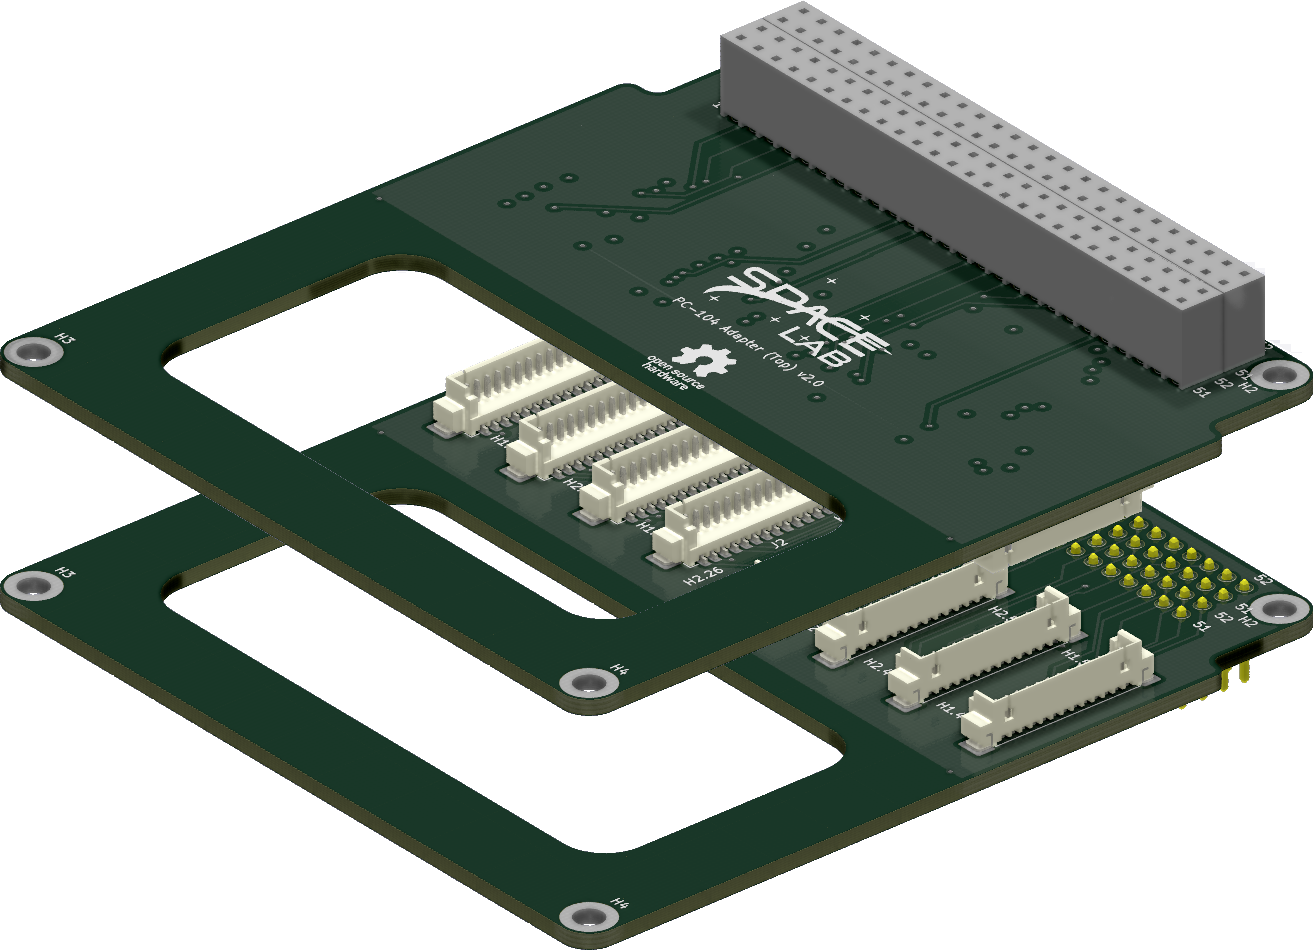
\includegraphics[width=0.7\textwidth]{figures/pc104-adapter}
        \caption{PC-104 adapter boards.}
        \label{fig:pc104-adapter}
    \end{center}
\end{figure}

\begin{figure}[!htb]
    \begin{center}
        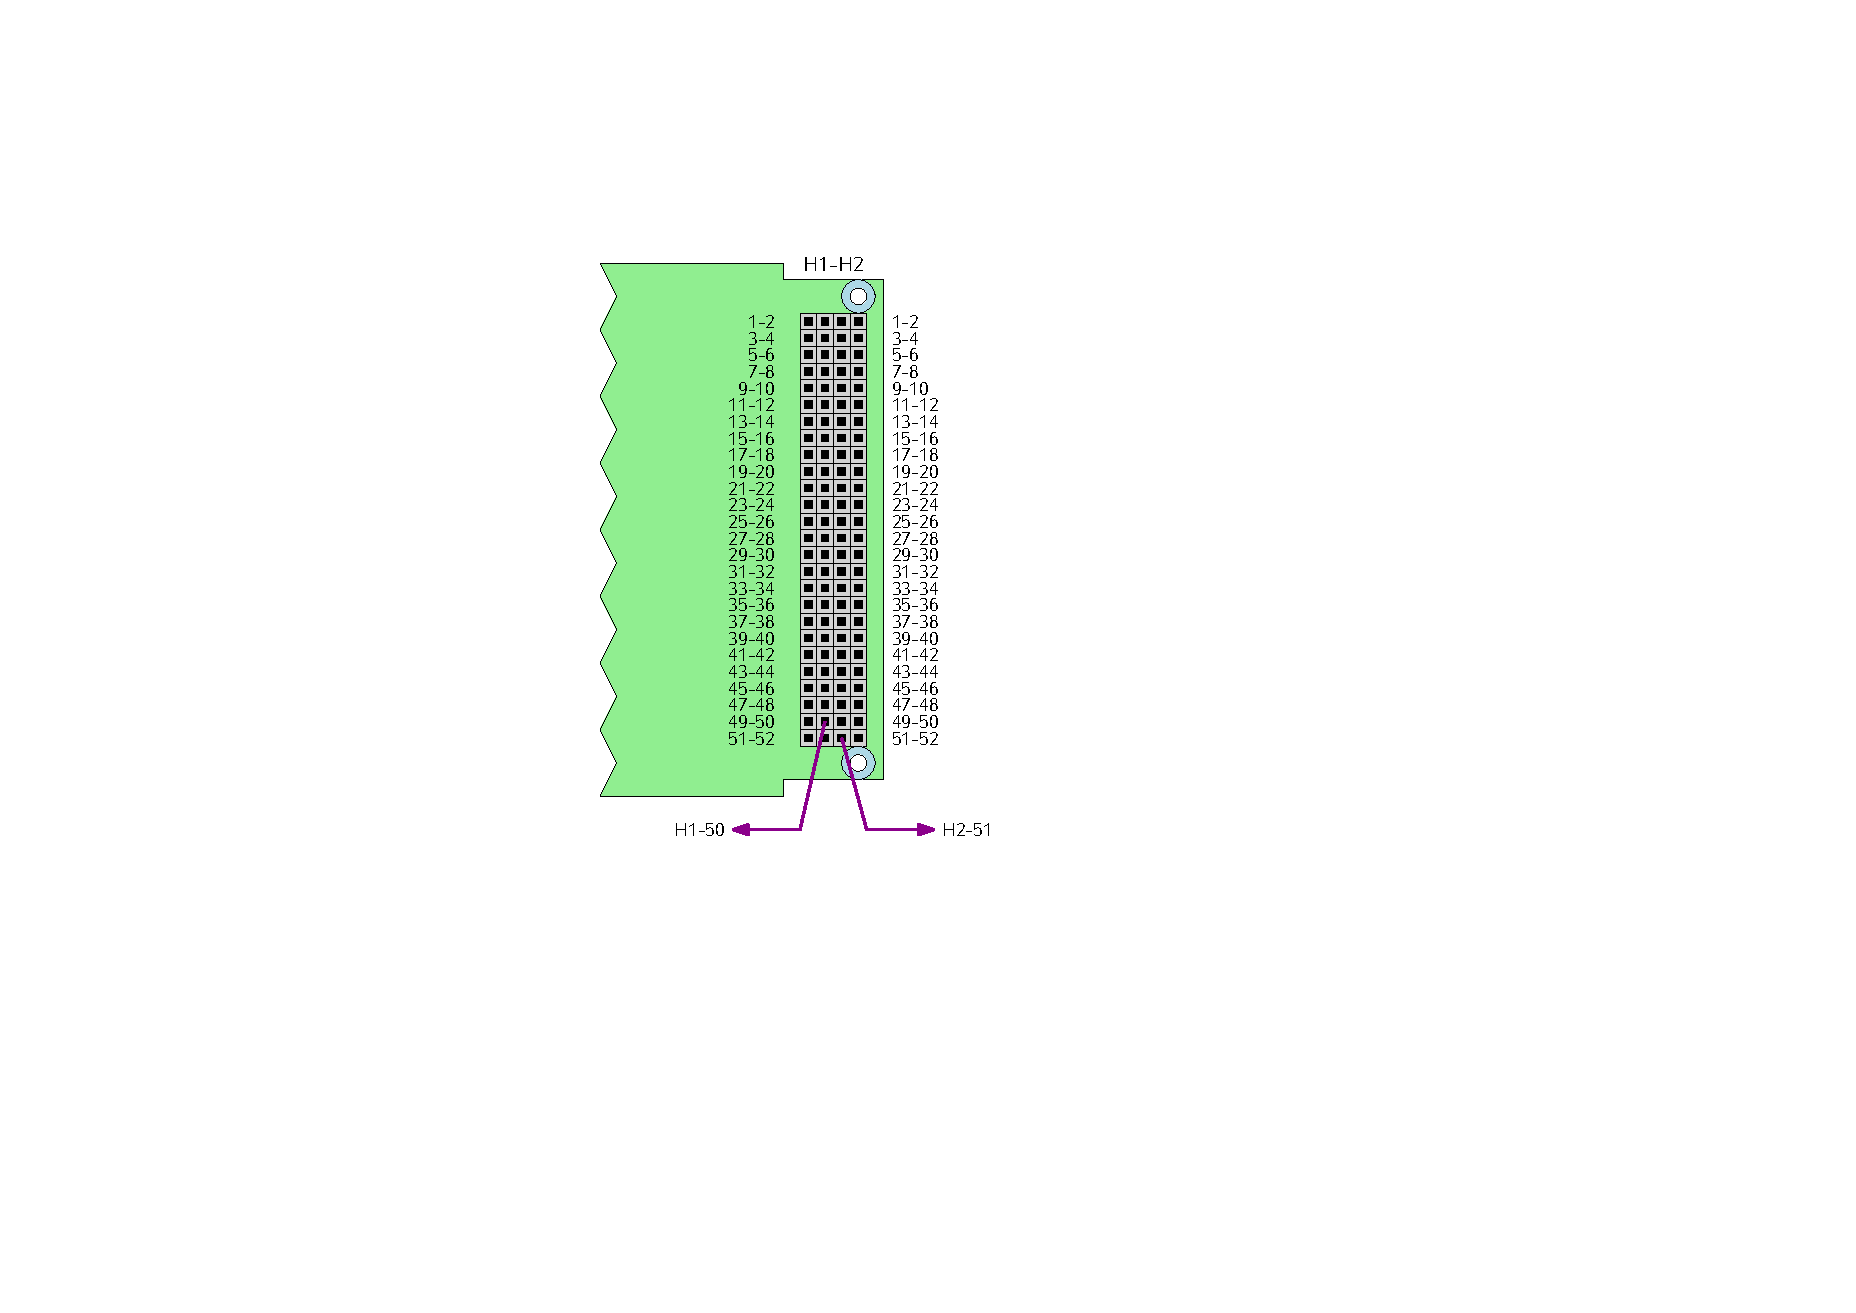
\includegraphics[width=0.45\textwidth]{figures/pc104-diagram}
        \caption{PC-104 pinout reference.}
        \label{fig:pc104-reference}
    \end{center}
\end{figure}

    %
% hardware.tex
%
% Copyright (C) 2020 by SpaceLab.
%
% PC-104 Adapter Documentation
%
% This work is licensed under the Creative Commons Attribution-ShareAlike 4.0
% International License. To view a copy of this license,
% visit http://creativecommons.org/licenses/by-sa/4.0/.
%

%
% \brief Hardware overview chapter.
%
% \author Gabriel Mariano Marcelino <gabriel.mm8@gmail.com>
%
% \institution Universidade Federal de Santa Catarina (UFSC)
%
% \version 2.0.0
%
% \date 2020/09/25
%

\chapter{Hardware Overview} \label{ch:hardware}

\cite{picoblade}

\section{Top Board}

\begin{figure}[!htb]
    \begin{center}
        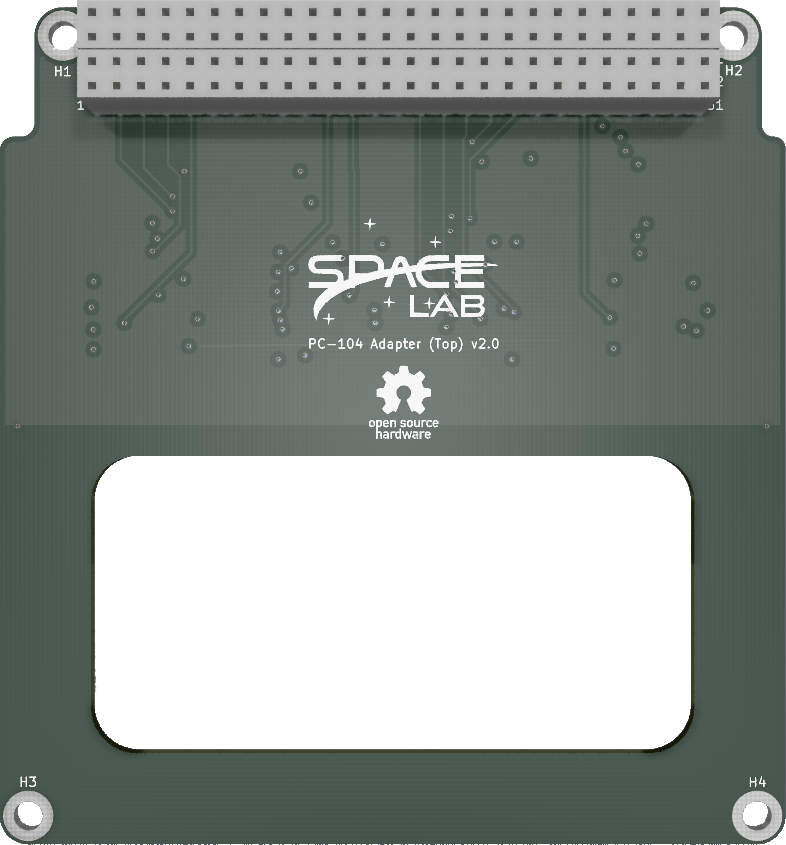
\includegraphics[width=8.636cm]{figures/pc104-adapter-top-top}
        \caption{Top view of the top board (real size).}
        \label{fig:top-board-top}
    \end{center}
\end{figure}

\begin{figure}[!htb]
    \begin{center}
        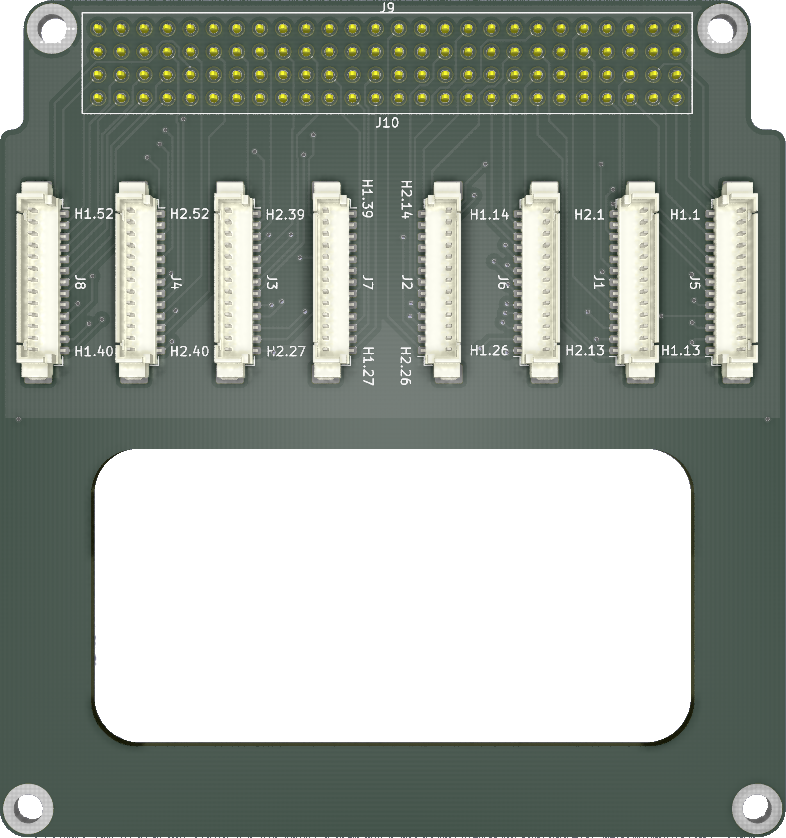
\includegraphics[width=8.636cm]{figures/pc104-adapter-top-bottom}
        \caption{Bottom view of the top board (real size).}
        \label{fig:top-board-bottom}
    \end{center}
\end{figure}

\section{Bottom Board}

\begin{figure}[!htb]
    \begin{center}
        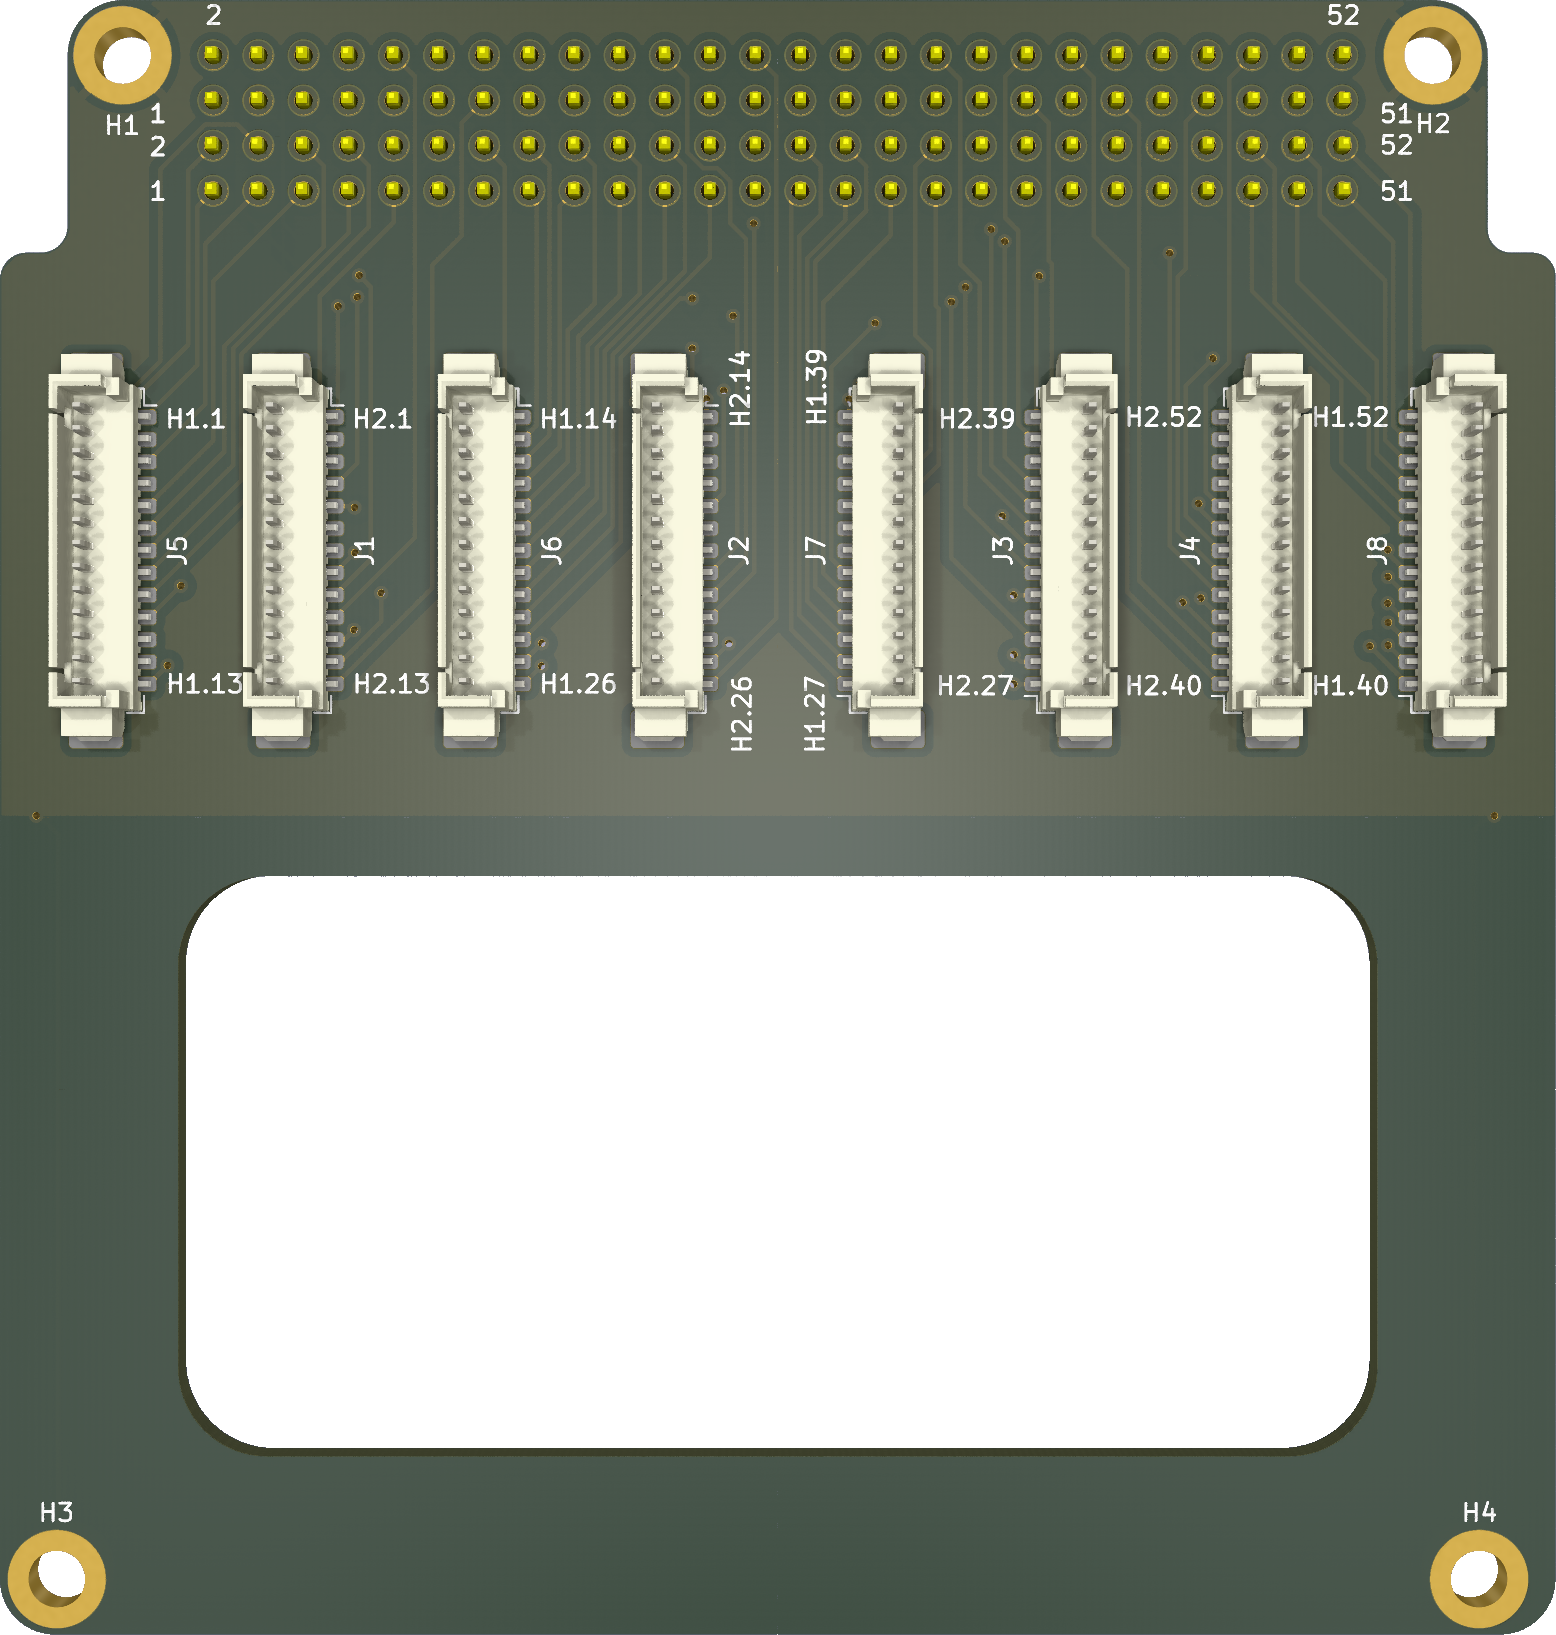
\includegraphics[width=8.626cm]{figures/pc104-adapter-bottom-top}
        \caption{Top view of the bottom board (real size).}
        \label{fig:bottom-board-top}
    \end{center}
\end{figure}

\begin{figure}[!htb]
    \begin{center}
        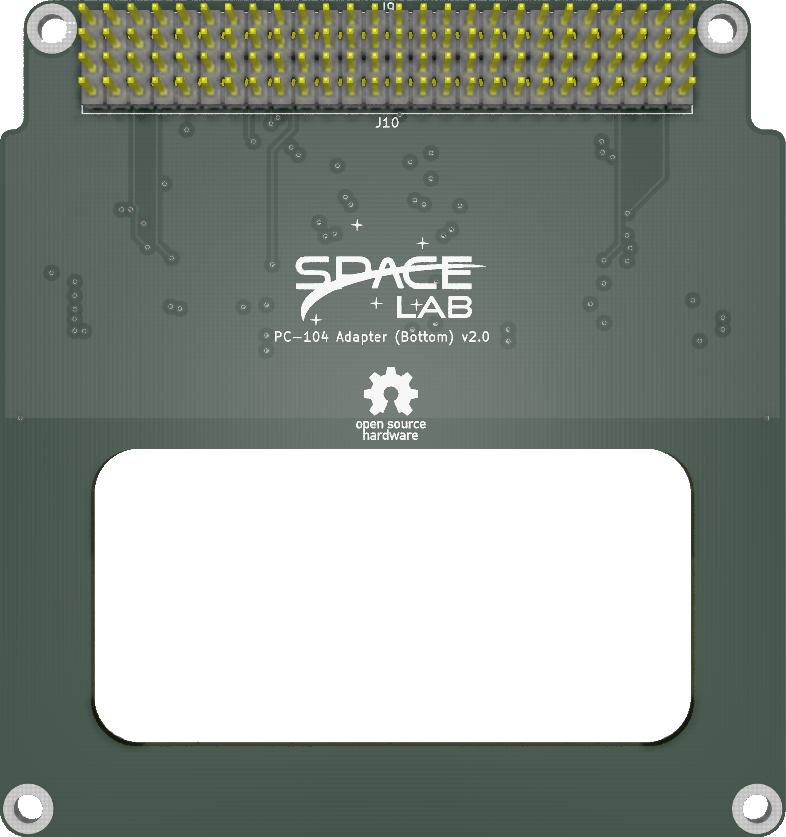
\includegraphics[width=8.626cm]{figures/pc104-adapter-bottom-bottom}
        \caption{Bottom view of the bottom board (real size).}
        \label{fig:bottom-board-bottom}
    \end{center}
\end{figure}

\section{Bill of Materials}

The Bill of Materials (BOM\nomenclature{\textbf{BOM}}{\textit{Bill Of Materials.}}) of the top and bottom boards are available in Tables \ref{tab:bom-top-board} and \ref{tab:bom-bottom-board}, respectively.

\begin{table}[!h]
    \centering
    \begin{tabular}{cllr}
        \toprule[1.5pt]
        \textbf{Item}   & \textbf{Designator}            & \textbf{Partnumber} & \textbf{Quantity} \\
        \midrule
        1               & J9, J10                        & SSW-126-01-G-D      & 2                 \\
        2               & J1, J2, J3, J4, J5, J6, J7, J8 & 53398-1371          & 8                 \\
        \bottomrule[1.5pt]
    \end{tabular}
    \caption{Bill of Materials (BOM) of the top board.}
    \label{tab:bom-top-board}
\end{table}

\begin{table}[!h]
    \centering
    \begin{tabular}{cllr}
        \toprule[1.5pt]
        \textbf{Item}   & \textbf{Designator}            & \textbf{Partnumber} & \textbf{Quantity} \\
        \midrule
        1               & J9, J10                        & TSW-126-07-G-D      & 2                 \\
        2               & J1, J2, J3, J4, J5, J6, J7, J8 & 53398-1371          & 8                 \\
        \bottomrule[1.5pt]
    \end{tabular}
    \caption{Bill of Materials (BOM) of the bottom board.}
    \label{tab:bom-bottom-board}
\end{table}

    %
% assembly.tex
%
% Copyright (C) 2020 by SpaceLab.
%
% PC-104 Adapter Documentation
%
% This work is licensed under the Creative Commons Attribution-ShareAlike 4.0
% International License. To view a copy of this license,
% visit http://creativecommons.org/licenses/by-sa/4.0/.
%

%
% \brief Assembly instructions chapter.
%
% \author Gabriel Mariano Marcelino <gabriel.mm8@gmail.com>
%
% \institution Universidade Federal de Santa Catarina (UFSC)
%
% \version 2.0.0
%
% \date 2020/10/19
%

\chapter{Assembly Instructions} \label{ch:assembly}

This chapter presents the assembly instructions of the two boards and the interconnection cables between the top and bottom boards.

This project does not have sensible components (electrostatic or temperature), and no major care should be taken during the solder process. A recommended temperature of the soldering iron can be 350 $^{\circ}$C or lower.

\section{Top Board}

\begin{enumerate}
    \item Solder the PicoBlade connectors (J1, J2, J3, J4, J5, J6, J7 and J8), beginning with the external connectors and moving to the center of the board, as can be seen in \autoref{fig:picoblades-instructions}.

\begin{figure}[!htb]
    \begin{center}
        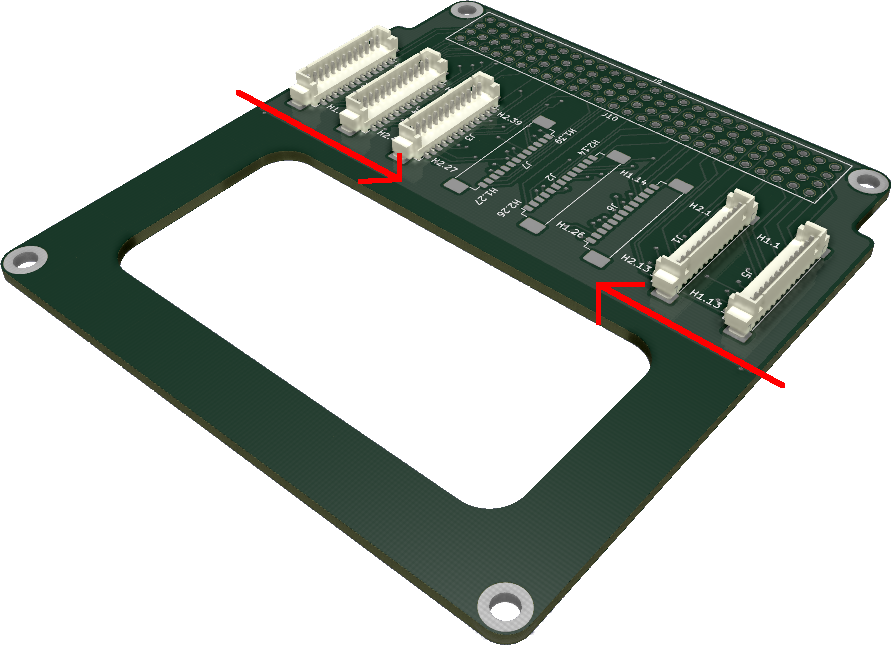
\includegraphics[width=0.6\columnwidth]{figures/picoblade-solder}
        \caption{Solder sequence of the PicoBlade connectors.}
        \label{fig:picoblades-instructions}
    \end{center}
\end{figure}

    \item Solder the PC-104 connectors (J9 and J10), taking care to keep the alignment of all the pins with the surface of the board, as can be seen in \autoref{fig:pc104-alignment}.

\begin{figure}[!htb]
    \begin{center}
        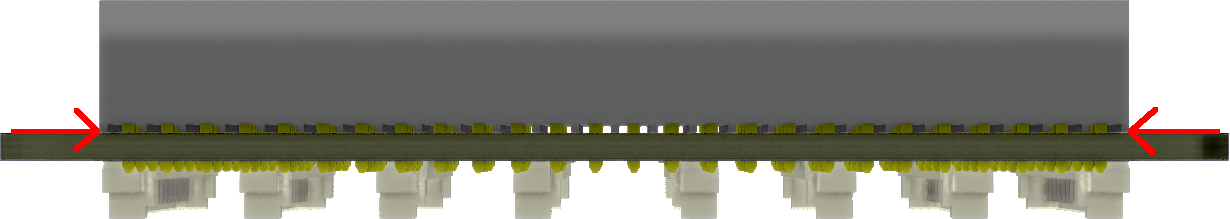
\includegraphics[width=0.7\columnwidth]{figures/pc104-alignment}
        \caption{Alignment of the PC-104 connectors.}
        \label{fig:pc104-alignment}
    \end{center}
\end{figure}
\end{enumerate}

\section{Bottom Board}

The same instructions apply to the bottom board:

\begin{enumerate}
    \item Solder the PicoBlade connectors (J1, J2, J3, J4, J5, J6, J7 and J8), beginning with the external connectors and moving to the center of the board, as can be seen in \autoref{fig:picoblades-instructions}.
    \item Solder the PC-104 connectors (J9 and J10), taking care to keep the alignment of all the pins with the surface of the board, as can be seen in \autoref{fig:pc104-alignment}.
\end{enumerate}

\section{Cables}

\begin{enumerate}
    \item .
\end{enumerate}

    %
% references.tex
%
% Copyright (C) 2020 by SpaceLab.
%
% PC-104 Adapter Documentation
%
% This work is licensed under the Creative Commons Attribution-ShareAlike 4.0
% International License. To view a copy of this license,
% visit http://creativecommons.org/licenses/by-sa/4.0/.
%

%
% \brief References chapter.
%
% \author Gabriel Mariano Marcelino <gabriel.mm8@gmail.com>
%
% \institution Universidade Federal de Santa Catarina (UFSC)
%
% \version 0.2.0
%
% \date 2020/06/21
%

\bibliography{references/pc104-adapter,references/picoblade,references/kicad}

\addcontentsline{toc}{chapter}{References}


\end{document}
